%\newpage
%%Машинист линии ведет бумажный журнал по выработке по заказам производства. В конце каждой смены мастер производства заносит сменный рапорт ПВА в систему 1С:УНФ. Мастер указывает выпуск продукции и расход заготовок в системе 1С:УНФ, распечатывает отчет производства и передает в бухгалтерию.

%В бухгалтерии на основании документа ''Заявка на приобретение'' (Рис. \ref{pic:d15}) создают документ «Производство».
%(рис. \ref{pic:a25}). 
%Бухгалтерия распределяет заготовки по заказам на производство. 


\newpage
\subsection{Ремонты и ППР}
\label{bp:maintance}


На предприятии создана ремонтная служба. Выделены должности главного инженера, главного механика и главного энергетика. В штат службы входят:
\begin{itemize}
    \item  Водитель, 1 чел.
    \item Слесарь-ремонтник, 7 чел (с учетом дежурных). 
    \item Токарь, 1 чел.
    \item Наладчик КИПиА, 4 чел.
    \item Электрик, 1 чел.
    \item Слесарь по ремонту и обслуживанию ПКС, 4 чел.
\end{itemize}

%Выделены должности инженеров по обслуживанию линий переработки и ГА.
Устранение аварийных простоев оборудования

При поломке оборудования бригадиры гофроагрегата и линий переработки ставят в известность начальника смены. Начальник смены вызывает необходимого специалиста ремонтной службы. В конце смены или по требованию начальника смены бригадир сообщает информацию о простоях по телефону и в чат WhatsApp. Ранее на линиях велись специальные журналы по оборудованию. На момент обследования журналы не ведутся. Дежурные в сменах журналы не ведут, существуют только чаты в WhatsApp. Статистика по простоям отсутствует.    

%Инженер по обслуживанию линий переработки каждое утро получает информацию по простоям у мастера смены и вносит их таблицу (рис. \ref{pic:f43}), которая выводится на монитор на производстве.  

%Инженер по обслуживанию линий переработки ведет расширенную таблицу по простоям и выработке оп каждому бригадиру и линии (рис. \ref{pic:a23}).



\textbf{Планирование и проведение ППР}

На предприятии создан график ППР (рис. \ref{pic:8 График ппр_0001}).  Но он не соблюдается из-за загрузки производства. Пробег оборудования отслеживается. Разработаны планы проведения ППР и смазки оборудования (рис. \ref{pic:8 план работ на ппр_0001}). На каждый ППР ремонтному персоналу выдаются задания (рис. \ref{pic:8 задание дежурному_0001}). Технологический персонал в момент проведения ППР занимается уборкой.  Технологические карты проведения ремонтов частично созданы, но большинство находится в разработке (рис. \ref{pic:8 ТК ремонта_0001}). Также в разработке находятся памятки "бегунки" для бригадиров гофроагрегата и линий переработки по осмотру оборудования.

\textbf{Заказ и получение ЗиП}

Созданы склады КИПиА и механики. Поиск необходимых запчастей осуществляется в интернете. Механик и энергетик самостоятельно связываются с поставщиками и получают коммерческие предложения, которые подписывает генеральный директор. Производится приобретение и оприходование ЗиП на склады. На складах ведется учет наличия минимального количества ЗиП, но возможны ситуации, когда ремонтный персонал не фиксирует что взяли со склада. %Инженер по обслуживанию линий переработки на ППР выдает задание на проведение ремонтных работ службам ОГЭ и ОГМ (рис. \ref{pic:a25},\ref{pic:a26}). Технологический персонал в момент проведения ППР занимается уборкой. Технологические карты по обслуживанию оборудования отсутствуют.
%График смазки по перерабатывающим линиям отсутствует.

%Инженер по обслуживанию ГА ведет журнал по неисправностям (рис. \ref{pic:f46}) и график смазки (рис. \ref{pic:f45}). Задание на ППР инженер по обслуживанию выдает в устной форме. Карты по обслуживанию ГА отсутствуют. 

%Для удобства замечания по работе ГА машинисты пишут на магнитной доске,
% (рис. \ref{pic:f47}), 
%расположенной на резках. На момент обследования замечания отсутствуют.

%Все расходные материалы по оборудованию меняют по мере износа после получения замечаний машинистов.
%Пробег оборудования не отслеживается.
\clearpage

\begin{figure}
\begin{center}
  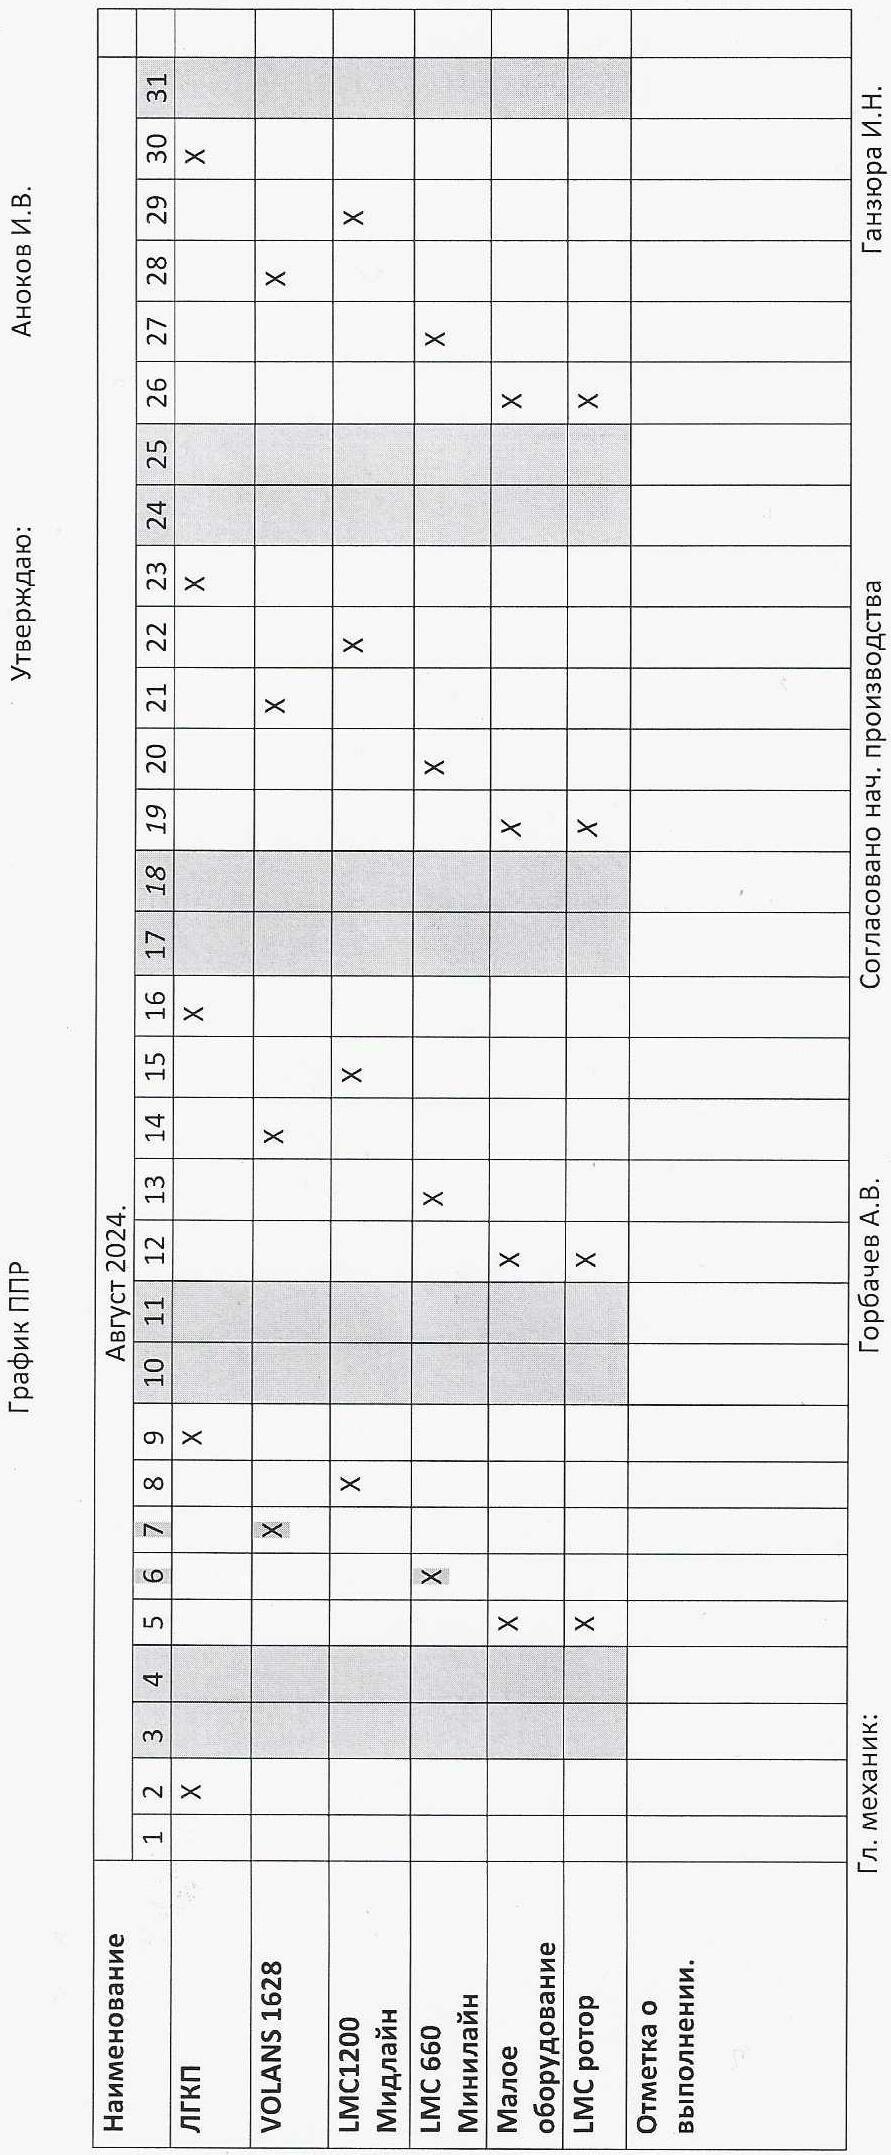
\includegraphics[height=0.94\textheight, width=0.94\textwidth, keepaspectratio]{Pics 1/8 График ппр_0001.jpg }
\end{center}
  \caption{График ППР}
  \label{pic:8 График ппр_0001}
\end{figure}

\begin{figure}
\begin{center}
  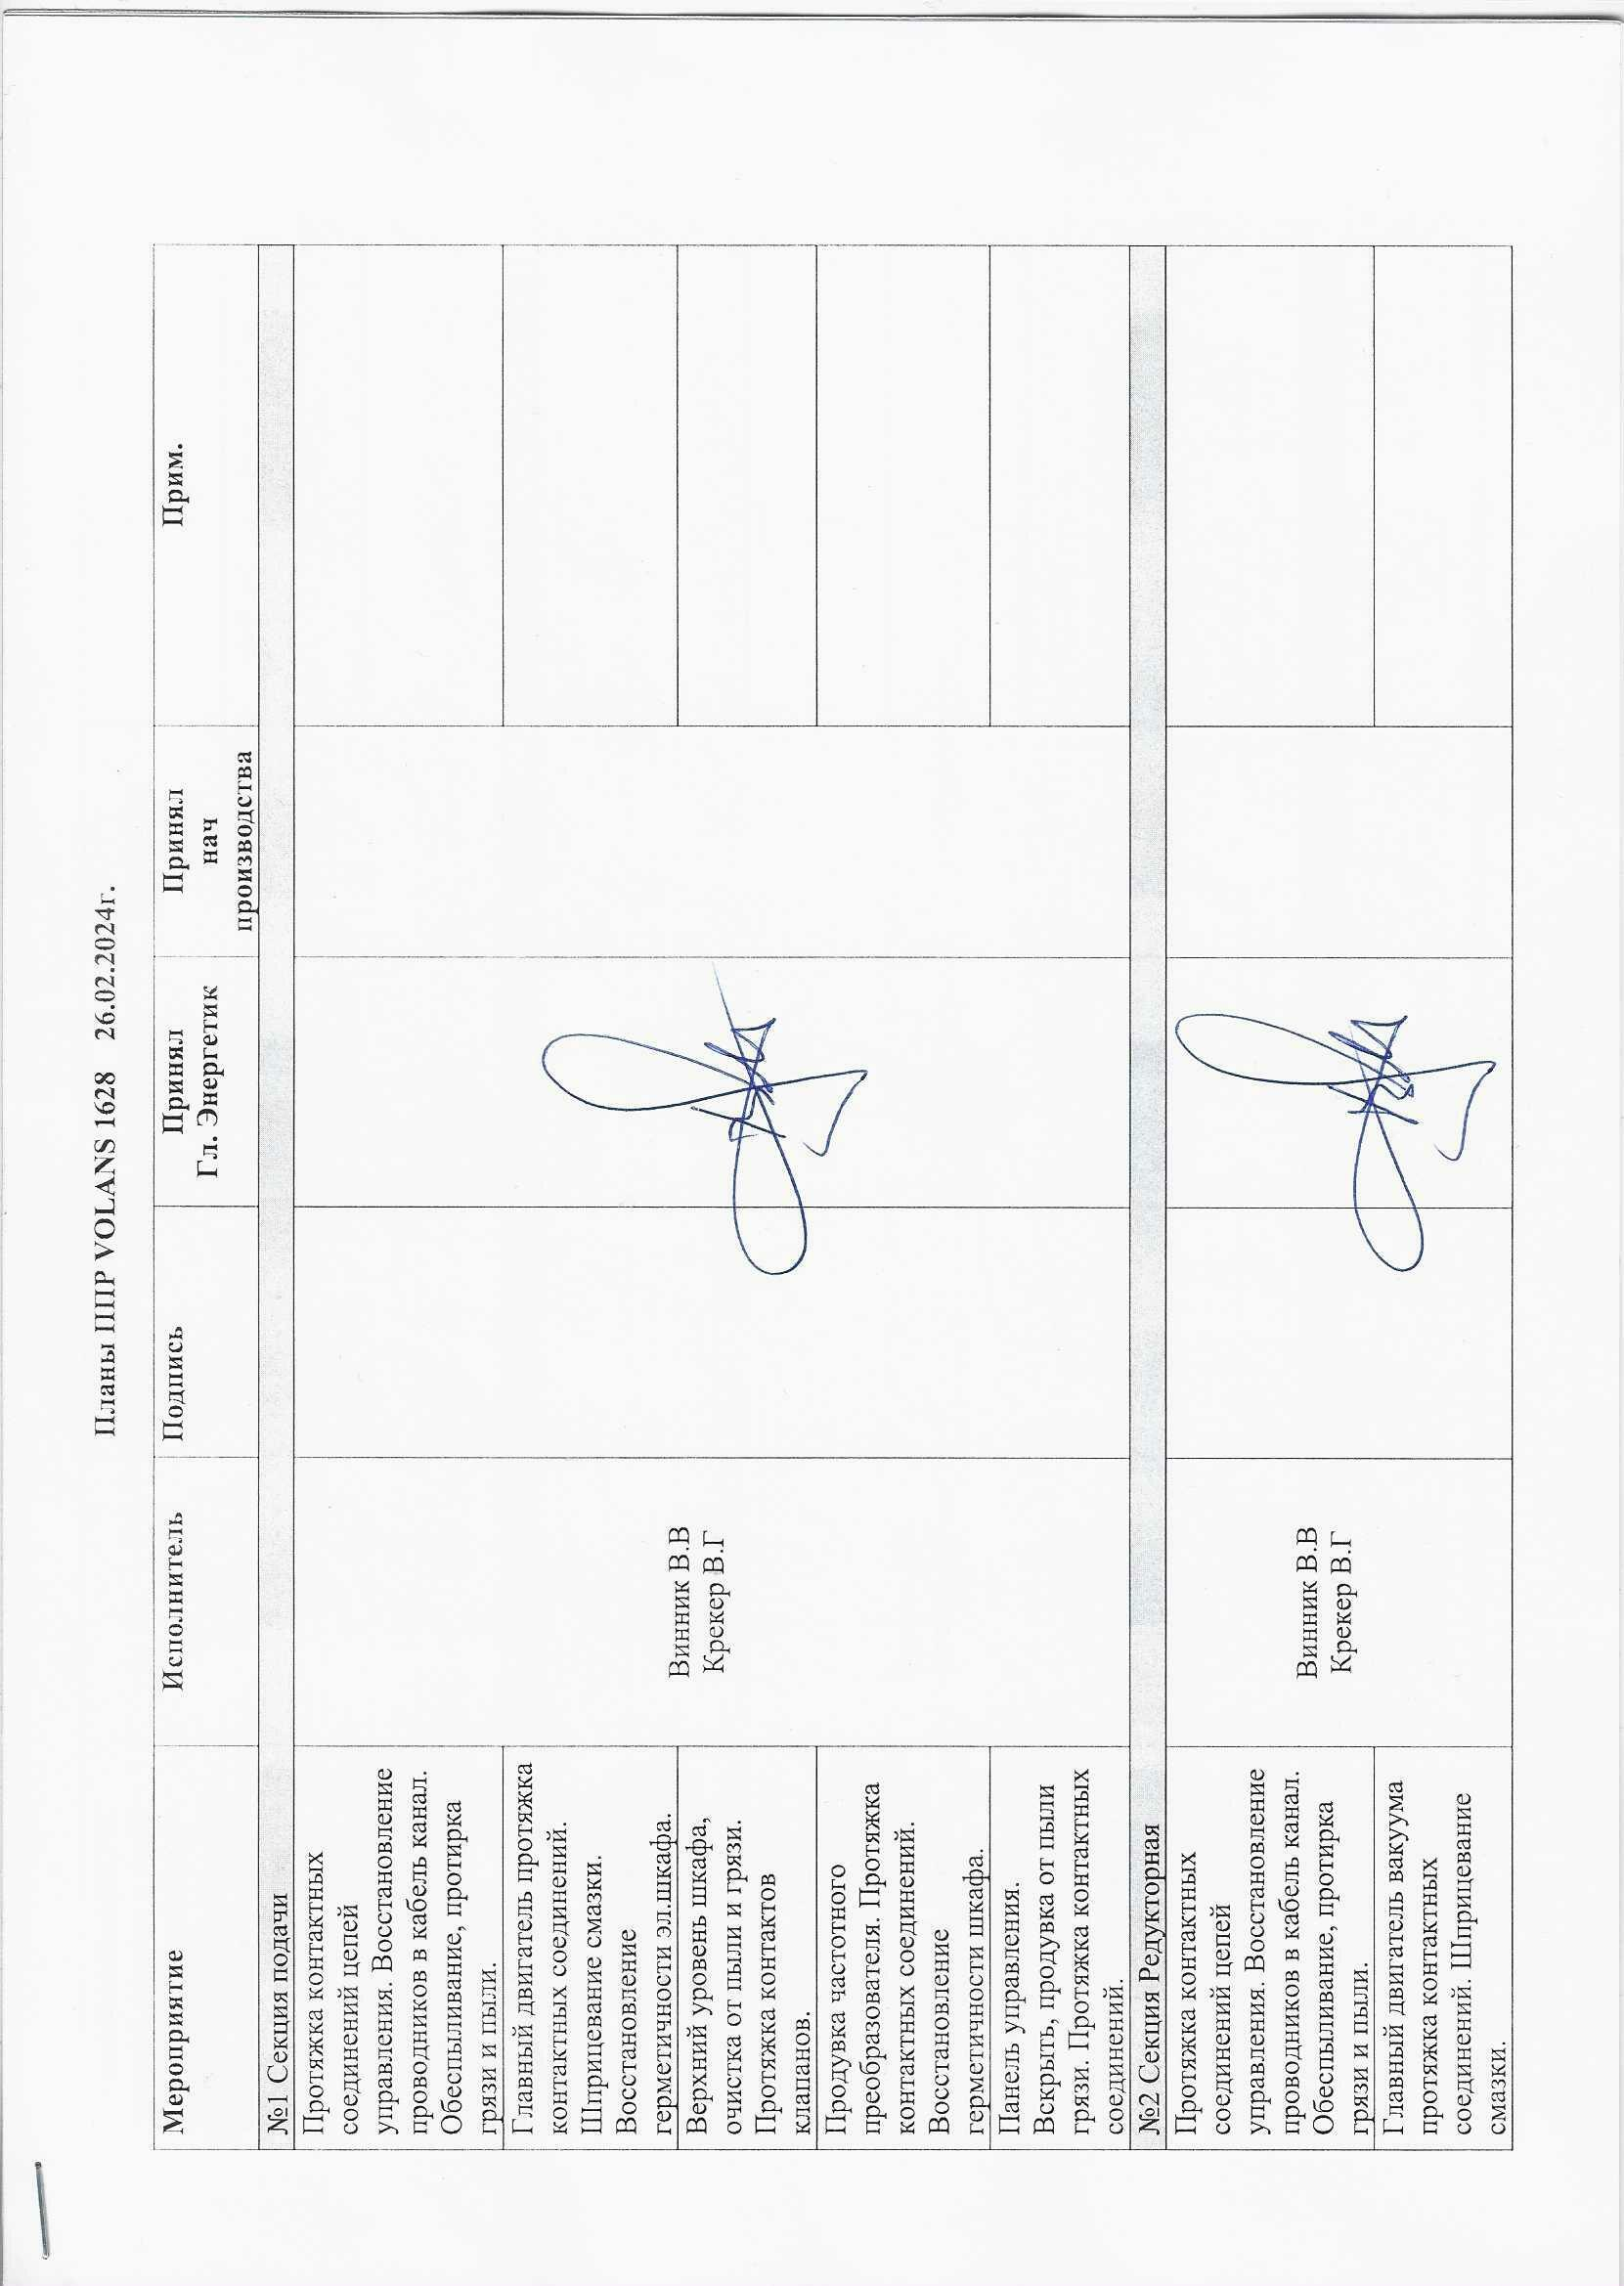
\includegraphics[height=0.94\textheight, width=0.94\textwidth, keepaspectratio]{Pics 1/8 план работ на ппр_0001.jpg }
\end{center}
  \caption{План работ на ППР}
  \label{pic:8 план работ на ппр_0001}
\end{figure}

\begin{figure}
\begin{center}
  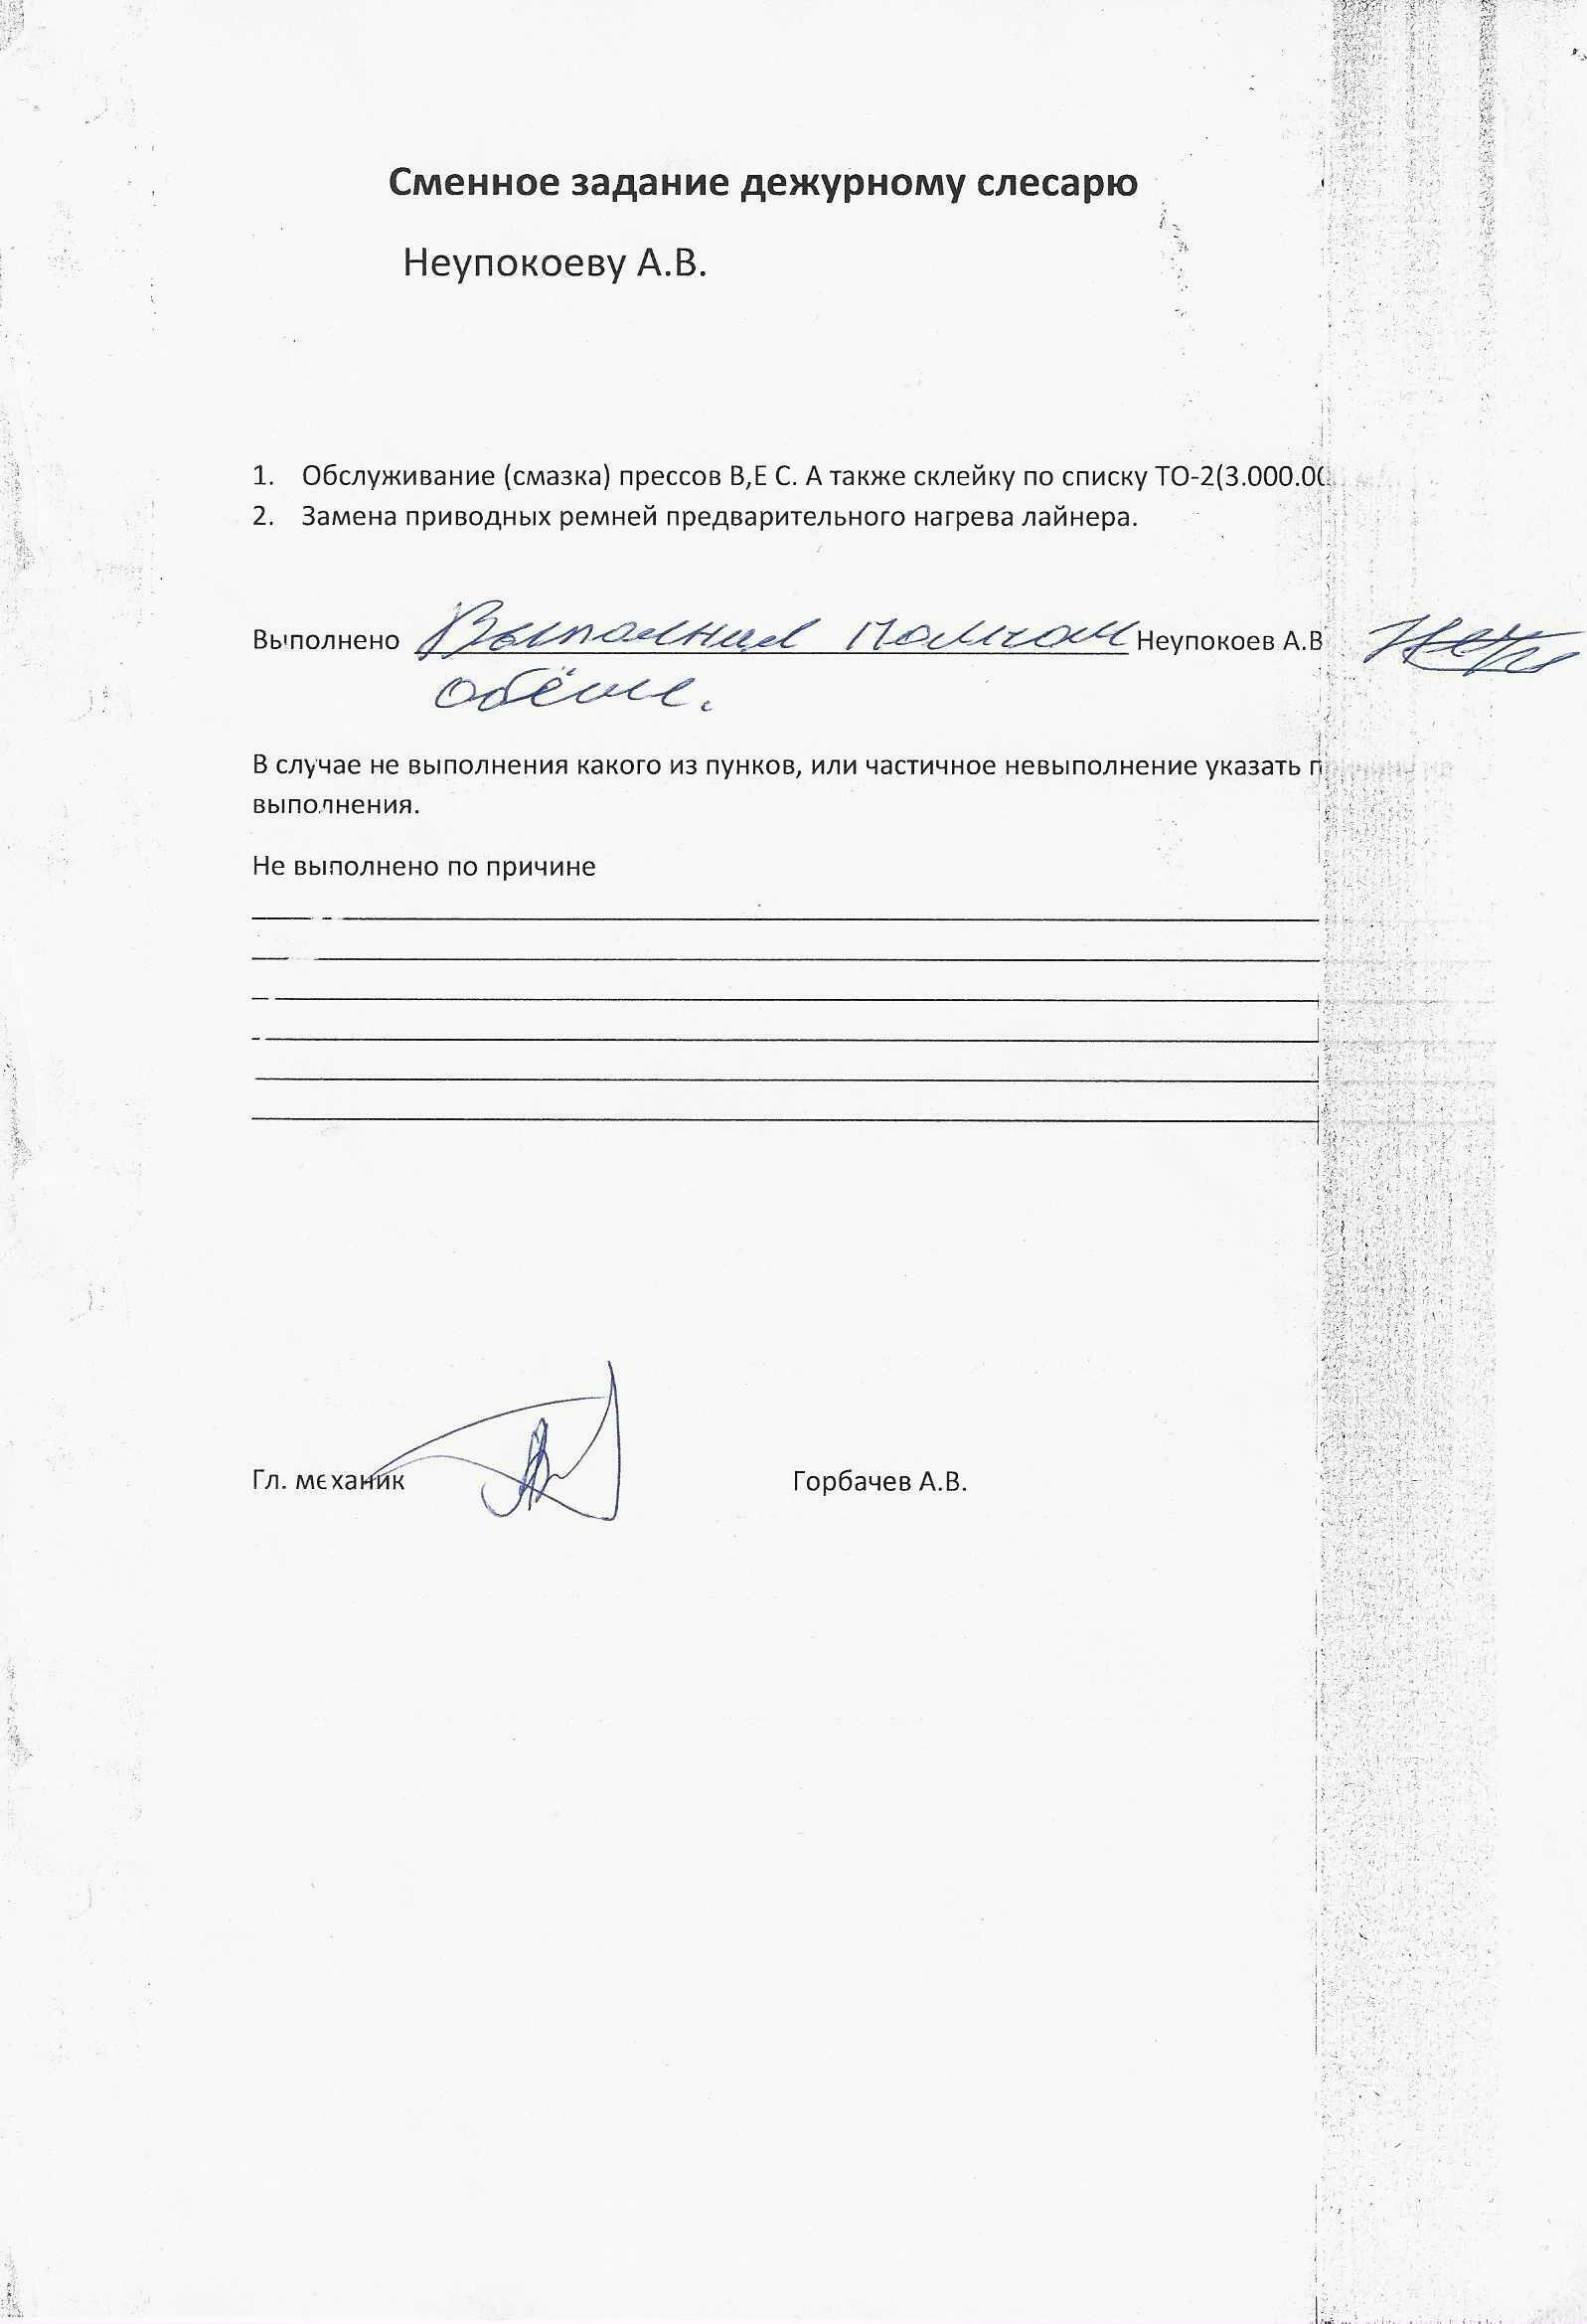
\includegraphics[height=0.94\textheight, width=0.94\textwidth, keepaspectratio]{Pics 1/8 задание дежурному_0001.jpg }
\end{center}
  \caption{Задание ремонтному персоналу}
  \label{pic:8 задание дежурному_0001}
\end{figure}



\begin{figure}
\begin{center}
  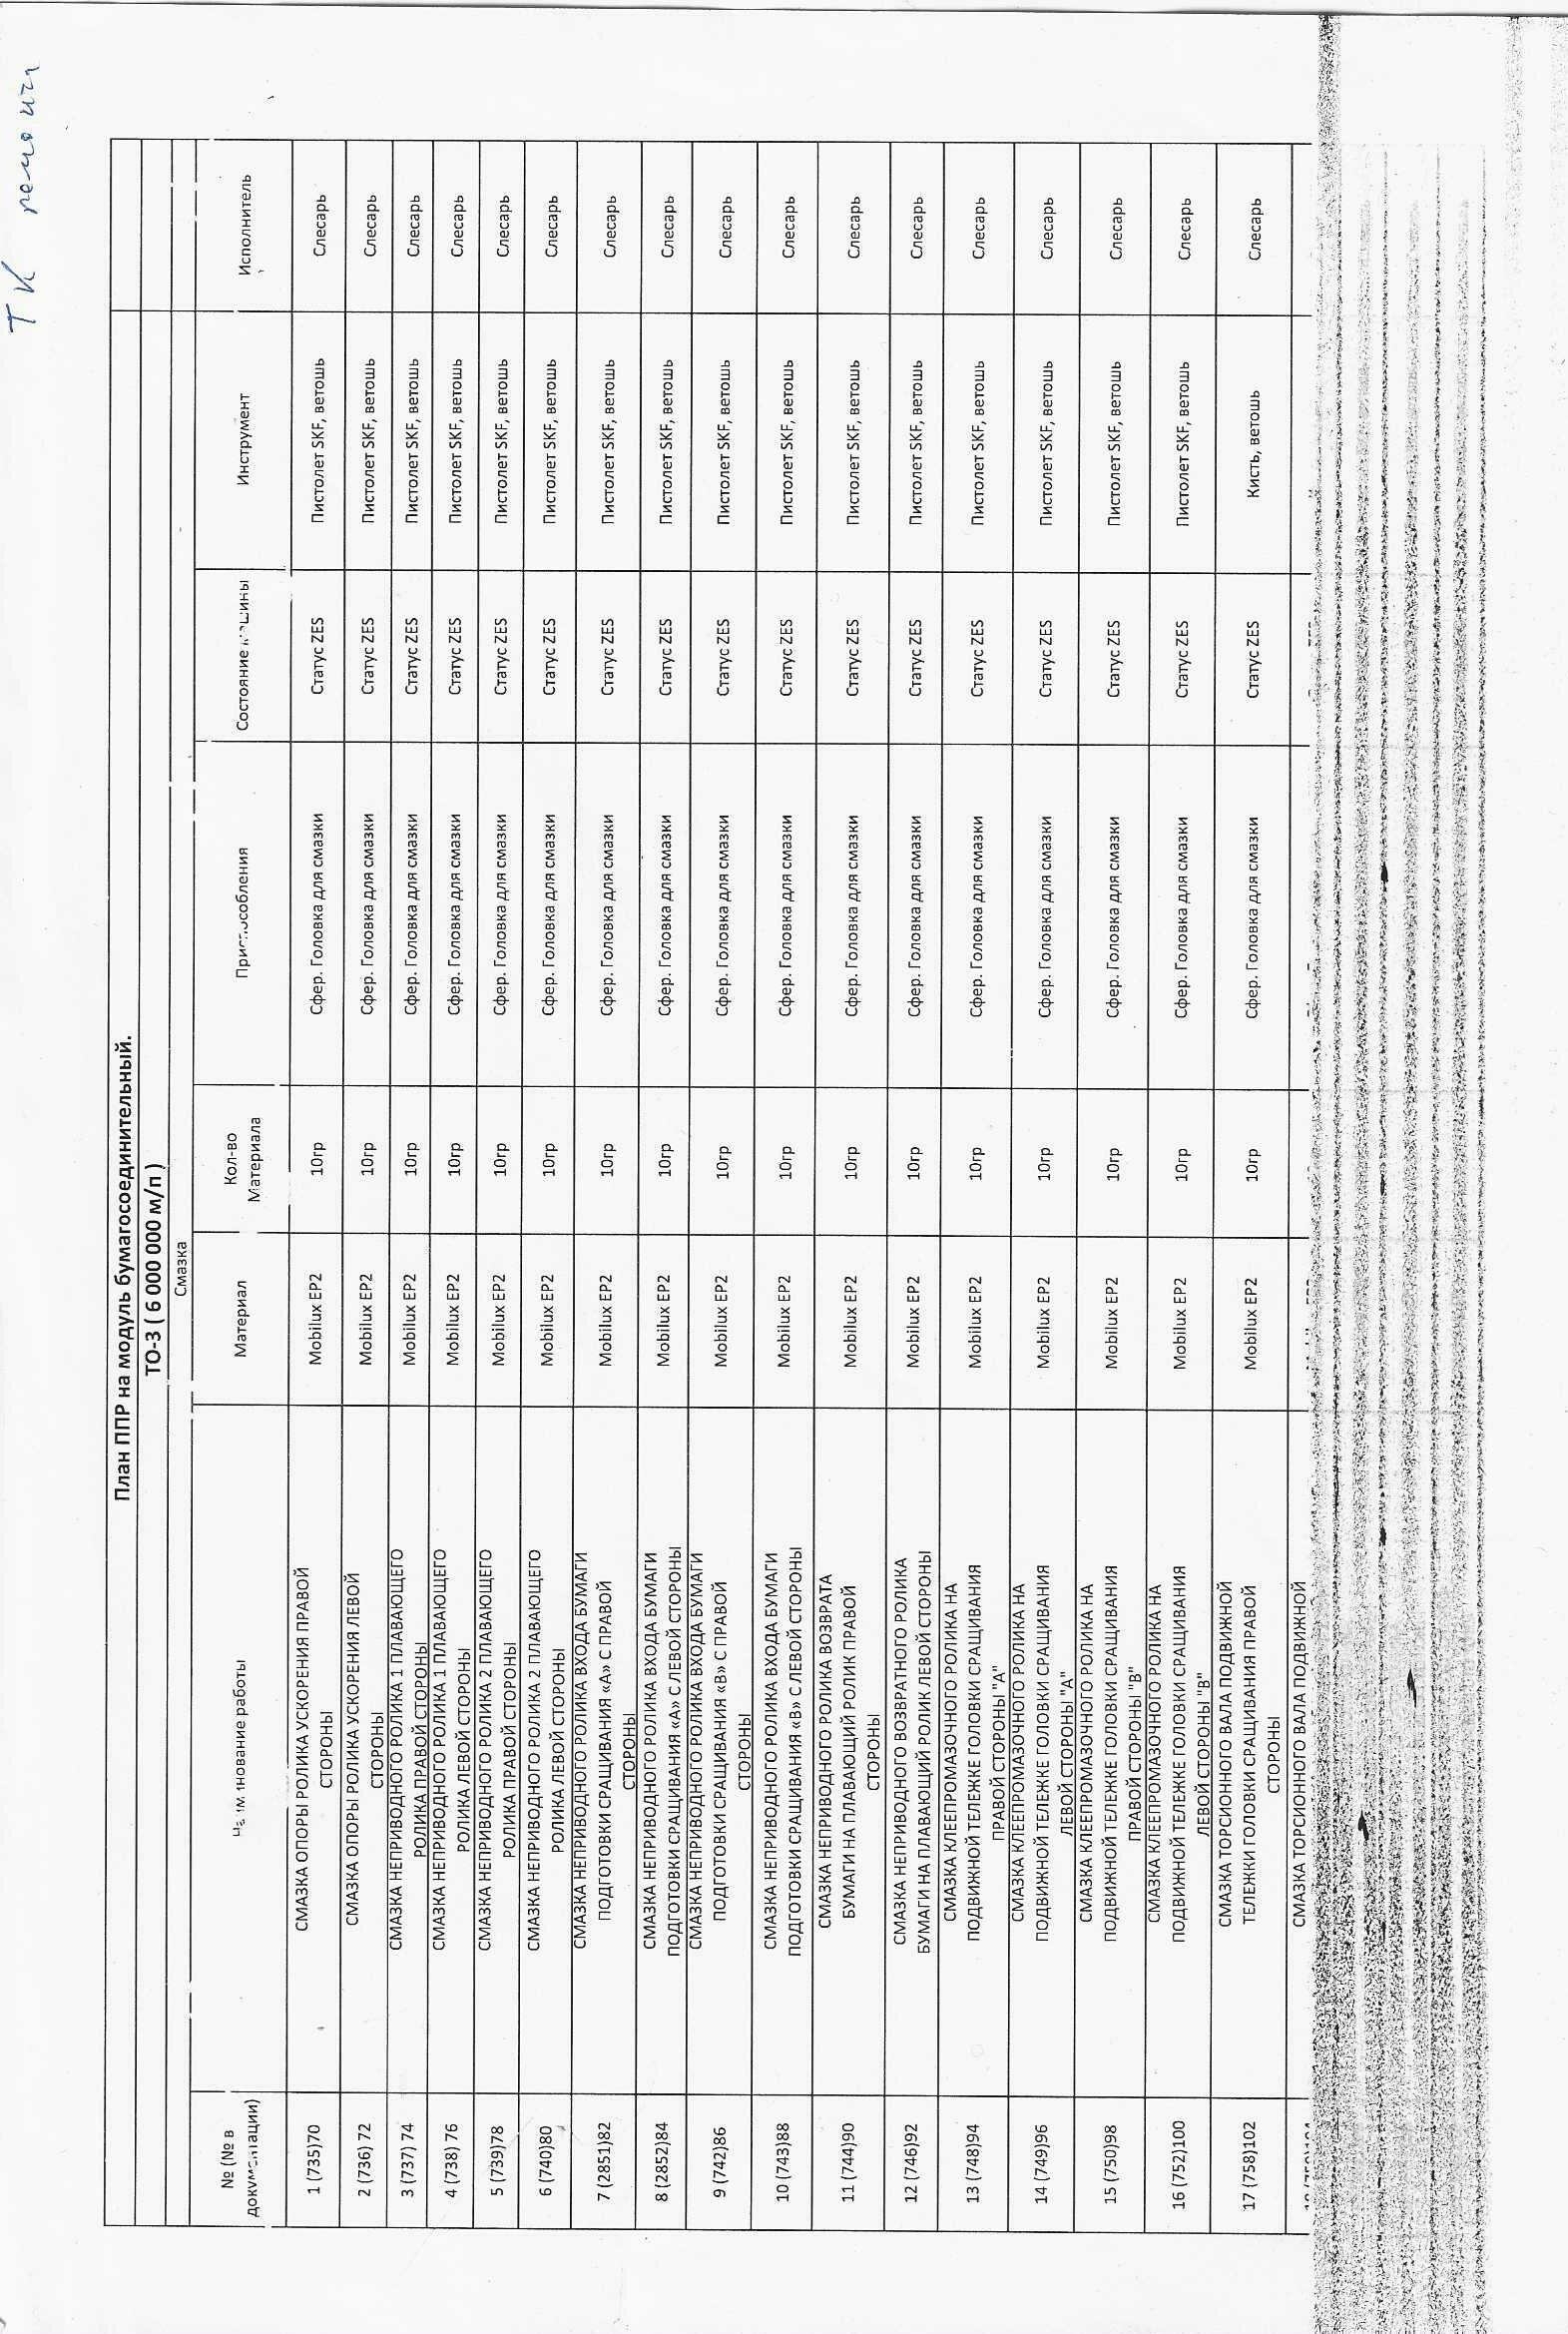
\includegraphics[height=0.94\textheight, width=0.94\textwidth, keepaspectratio]{Pics 1/8 ТК ремонта_0001.jpg }
\end{center}
  \caption{Технологическая карта ремонта}
  \label{pic:8 ТК ремонта_0001}
\end{figure}

\clearpage
%%Мелкий ремонт делают сразу при обнаружении. Более крупный ремонт планируют на совещаниях. Ведутся записи по крупным поломкам и недочетам (рис. \ref{pic:a34}). Каждый день проводят совещания и ведется протокол, куда вписывают в том числе недочеты по оборудованию, сроки устранения и ответственных. 
% (рис. \ref{pic:a77}). 

%Запчасти заказывает директор по производству и инженер-технолог. Есть склад запчастей (рис. \ref{pic:a42}) и ведется реестр по запчастям (рис. \ref{pic:a43}). Инженер-технолог списывает запчасти по актам раз в месяц.


%В%едется журнал замечаний (рис.
% \ref{pic:a38}, 
%\ref{pic:a39}). На момент обследования последние замечания были без подписей. 

%Со слов директора по производству, смазку оборудования проводят еженедельно, документальное подтверждение отсутствует.

%Есть план проведения ППР технологическим персоналом, в котором расписаны работы по уборке оборудования  (рис. \ref{pic:a35}).  Работ по обслуживанию оборудования не обнаружено.
% , \ref{pic:a36}, \ref{pic:a37}).


% \begin{figure}
% \begin{center}
%   \includegraphics[height=0.94\textheight, width=\textwidth, keepaspectratio]{Pics/a63.jpg}
% \end{center}
%   \caption{Журнал измерений качества заготовок}
%   \label{pic:a63}
% \end{figure}



% \begin{figure}
% \begin{center}
%  \includegraphics[height=0.4\textheight, keepaspectratio]{Pics/f47.jpg}
% \end{center}
%  \caption{Замечания по работе оборудования}
%  \label{pic:f47}
% \end{figure}